\graphicspath{{./chapters/chapter3/}}
%\newtheorem*{rep@theorem}{\rep@title}
%\newcommand{\newreptheorem}[2]{%
%\newenvironment{rep#1}[1]{%
% \def\rep@title{#2 \ref{##1}}%
% \begin{rep@theorem}}%
% {\end{rep@theorem}}}
%\makeatother
%%\newtheorem{thm}{Theorem}
%\newreptheorem{thm}{Theorem}
%%\newtheorem{lem}[thm]{Lemma}
%\newreptheorem{lem}{Lemma}
%\newtheorem{prop}[thm]{Proposition}
%\newreptheorem{prop}{Proposition}
%%\newtheorem{cor}[thm]{Corollary}
%\newreptheorem{cor}{Corollary}
%\newtheorem{claim}{Claim}
%
%\newtheorem{innercustomgeneric}{\customgenericname}
%\providecommand{\customgenericname}{}
%\newcommand{\newcustomtheorem}[2]{%
%  \newenvironment{#1}[1]
%  {%
%   \renewcommand\customgenericname{#2}%
%   \renewcommand\theinnercustomgeneric{##1}%
%   \innercustomgeneric
%  }
%  {\endinnercustomgeneric}
%}
%
%\newcustomtheorem{customthm}{Theorem}
%\newcustomtheorem{customlemma}{Lemma}
%\newcustomtheorem{customprop}{Proposition}
%
%\newcommand{\defref}[1]{Definition~\ref{#1}}
%\newcommand{\tabref}[1]{Table~\ref{#1}}
%\newcommand{\figref}[1]{Fig.~\ref{#1}}
%\newcommand{\eqnref}[1]{\text{Eq.}~(\ref{#1})}
%\newcommand{\secref}[1]{\textnormal{Section}~\ref{#1}}
%\newcommand{\appref}[1]{Appendix \ref{#1}}
%\newcommand{\stepref}[1]{Step \ref{#1}}
%% \newcommand{\appref}[1]{the Appendix} % for short version of the paper
%\newcommand{\thmref}[1]{Theorem~\ref{#1}}
%\newcommand{\corref}[1]{Corollary~\ref{#1}}
%\newcommand{\propref}[1]{Proposition~\ref{#1}}
%\newcommand{\lemref}[1]{Lemma~\ref{#1}}
%\newcommand{\conref}[1]{Condition~\ref{#1}}
%\newcommand{\assref}[1]{Assumption~\ref{#1}}
%%\newcommand{\algref}[1]{Algorithm~\ref{#1}}
%\newcommand{\egref}[1]{Example~\ref{#1}}
%\newcommand{\algoref}[1]{Algorithm~\ref{#1}}
%
%\newcommand{\op}[1]{\operatorname{#1}}
%\newcommand{\paren} [1] {\ensuremath{ \left( {#1} \right) }}
%\newcommand{\parenb} [1] {\ensuremath{ \big( {#1} \big) }}
%\newcommand{\bigparen} [1] {\ensuremath{ \Big( {#1} \Big) }}
%\newcommand{\biggparen} [1] {\ensuremath{ \bigg( {#1} \bigg) }}
%\newcommand{\Biggparen} [1] {\ensuremath{ \Bigg( {#1} \Bigg) }}
%\newcommand{\bracket}[1]{\left[#1\right]}
%\newcommand{\tuple}[1]{\ensuremath{\left\langle #1 \right\rangle}}
%%\newcommand{\set}[1]{\ensuremath{\left\{#1\right\}}}
%\newcommand{\curlybracket}[1]{\ensuremath{\left\{#1\right\}}}
%\newcommand{\norm}[2]{\ensuremath{\left\langle#1,\:#2\right\rangle_{\cH_{\rK}}}}
%\newcommand{\normg}[2]{\ensuremath{\left\langle#1,\:#2\right\rangle}}
%\newcommand{\condcurlybracket}[2]{\ensuremath{\left\{#1\left\lvert\:#2\right.\right\}}}
%\newcommand{\inmod}[1]{\ensuremath{\left\lvert\left\lvert#1\right\rvert\right\rvert}}
%\newcommand{\boldalpha}{\ensuremath{\boldsymbol{\alpha}}}

\def\ind{\mathbbm{1}}
\def\oc{Online\_Cluster}
\def\ocns{No\_Sub\_Cluster}
\def\mem{\mathcal M}
\def\E{\mathbb{E}}
\def\R{\mathbb{R}}
\def\OC{\text{OC}}
\def\cH{\mathcal H}
\def\reals{\mathbb{R}}
\def\cD{\mathcal D}
\def\Ev{\mathbb{E}}
\def\cO{\mathcal O}
\def\cX{\mathcal X}
\def\cU{\mathcal U}
\def\cM{\mathcal M}



\chapter{Appendix for Chapter 4}

\section{Details for the proof of Theorem \ref{thm:lower_bound1}}\label{sec:lower_bound_proof}

\begin{proof}
We want to show that for any $m \in \mathbb{N}$, any learner on $m$ samples must fail with constant probability. Toward this end, set $M = \binom{3m}{m}$, and let $Z^{(M)}_1, Z^{(M)}_2, \dots, Z^{(M)}_M$ be subsets of $\R^d$ as described by Lemma \ref{lem:finding_shatter} (we will drop the superscript in what follows). Let $\mathcal{M}$ denote the set of all subsets of $\{1, \dots, 3m\}$ with exactly $m$ elements. Associate with each $Z_i$ a unique element of $\mathcal{M}$, thus allowing us to rename our subsets as $\{Z_T: T \in \mathcal{M}\}.$ We will now construct a set of robustness regions $U$ from these subsets. For $1 \leq i \leq 3m$, define $$U_{x_i} = \cup_{T: i \in T} Z_T,$$ where $x_i$ is an arbitrary point inside $U_{x_i}$. Note this is well-defined since the $Z^{(M)}$ are mutually disjoint.

By Lemma \ref{lem:finding_shatter}, it follows that if all $x_i$ are given a label of $-1$, then any classifier $h \in \cH_W$ satisfies that $h(z) = 1$ for some subset $T$ and some $z \in Z_T$. However, this will imply that $h$ lacks robustness on all $x \in \{x_i: i \in T\}$, meaning that there are at least $m$ points among $\{x_1, \dots, x_{3m}\}$ where $h$ has robust loss $1$. Furthermore, the second part of Lemma \ref{lem:finding_shatter} implies that for any $T \in \mathcal{M}$, there exists a classifier $h_T$ for which $h_S$ is $-1$ over all $Z_{T'}$ for $T' \neq T$. This implies that $h_T$ is robust at all $x_i$ \textit{except} for $x_i$ with $i \in S$. 

With these observations, we are now prepared to show that for any learner $L$, there exists a distribution $D$ for which $L$ has large expected robust loss. To do this, we use a standard lower bound technique found in \cite{ml_book} that was adapted to the robust setting in \cite{Srebro19}.

 The idea will be to pick $D$ to be the uniform distribution over a random subset of $2m$ points in $\{x_1, \dots, x_{3m}\}$. We will then argue that because $L$ only has access to $m$ points from $D$, it won't be able to distinguish which subset $D$ corresponds to, and this will lead to a large expected loss.

To this end, for any $T \in \cM$, let $D_T$ be the data distribution over $\R^d \times \{\pm 1\}$ where $x$ is chosen at uniform from $\{x_i: i \notin T\}$ and $y$ is always $-1$. We may assume without loss of generality that our learning algorithm, $L$, always outputs a classifier among the set $\{h_T: T \in \cM\}$. This is because Lemma \ref{lem:finding_shatter} implies that any classifier in $h \in \cH_W$ has robust loss that is at least as bad some $h_T$ (namely, if the decision boundary of $h$ crosses $Z_T$). 

Next, let $T, T' \in \cM$ be arbitrary. By definition, $h_T$ lacks robustness on all $x_i$ with $i \in T$, and is perfectly accurate and robust at all other points. It follows that among the $2m$ points in the support of $D_{T'}$, there are $m - |T \cap T'|$ where $h_T$ lacks robustness, implying the the loss of classifier $h_T$ with respect to distribution $D_{T'}$ is $\frac{1}{2} - \frac{|T \cap T'|}{2m}$. Note that this implies that $h_T$ has $0$ robust loss over $D_T$ (thus meeting the first stipulation of Theorem \ref{thm:lower_bound1}). 

Finally, we bound the expected loss of the learner $L$ with respect to a uniformly random choice of $D_T$. Let $\cM$ also denote the uniform distribution over itself, and let $\cU$ denote the uniform distribution over $\{1, 2, 3, \dots, 3m\}$. Taking expectations over $T \sim \cM$ and $S \sim D_T^m$, and letting $h_{L(S)}$ denote the classifier learned by $L$, we have that 
\begin{equation*}
\begin{split}
\E_{T \sim \cM} \E_{S \sim D_T^m} \left[\ell_U(h_{L(S)}, D_T)\right] &= \E_{S \sim \cU^m} \E_{T \sim (\cM | S)} \left[\ell_U(h_{L(S)}, D_T)\right] \\
&= \E_{S \sim \cU^m} \E_{T \sim \{T': T' \in \cM, S \cap T' = \emptyset\}}\left[ \frac{1}{2} - \frac{|T \cap L(S)|}{2m} \right].\\
\end{split}
\end{equation*}
To bound the inner expectation, observe that since $|S| = m$, $T'$ has a conditional distribution that is an arbitrary (at uniform) subset of at least $2m$ indices. Since $L(S)$ is fixed, it follows that the probability that any element in $L(S)$ is an element of $T'$ is at most $\frac{1}{2}$, meaning that the expected value of $|T \cap L(S)|$ is at most $\frac{|L(S)|}{2} = \frac{m}{2}$. Substituting this, we have that 
\begin{equation*}
\begin{split}
\E_{T \sim \cM} \E_{S \sim D_T^m} \left[\ell_U(h_{L(S)}, D_T)\right] \geq \E_{S \sim \cU^m} \E_{T \sim \{T': T' \in \cM, S \cap T' = \emptyset\}}\left[ \frac{1}{2} - \frac{m}{4m} \right] = \frac{1}{4}.\\
\end{split}
\end{equation*}
By Markov's inequality, any random variable between $0$ and $1$ with expectation $\frac{1}{4}$ is strictly larger than $\frac{1}{8}$ with probability at least $\frac{1}{7}$. Since the loss above is bounded between $0$ and $1$, it follows that $\Pr_{T \sim \cM}\Pr_{S \sim D_T} [\ell_U(h_{L(S)}, D) > \frac{1}{8}] \geq \frac{1}{7}$. Thus, for some $D = D_T$, the desired claim holds, finish the proof.
\end{proof}

\section{Sample Oracle Lower Bounds}\label{app: lower bound}
\begin{figure}[h!]
\centering
	%\begin{subfigure}[b]{0.11\textwidth}
	 %  \centering
		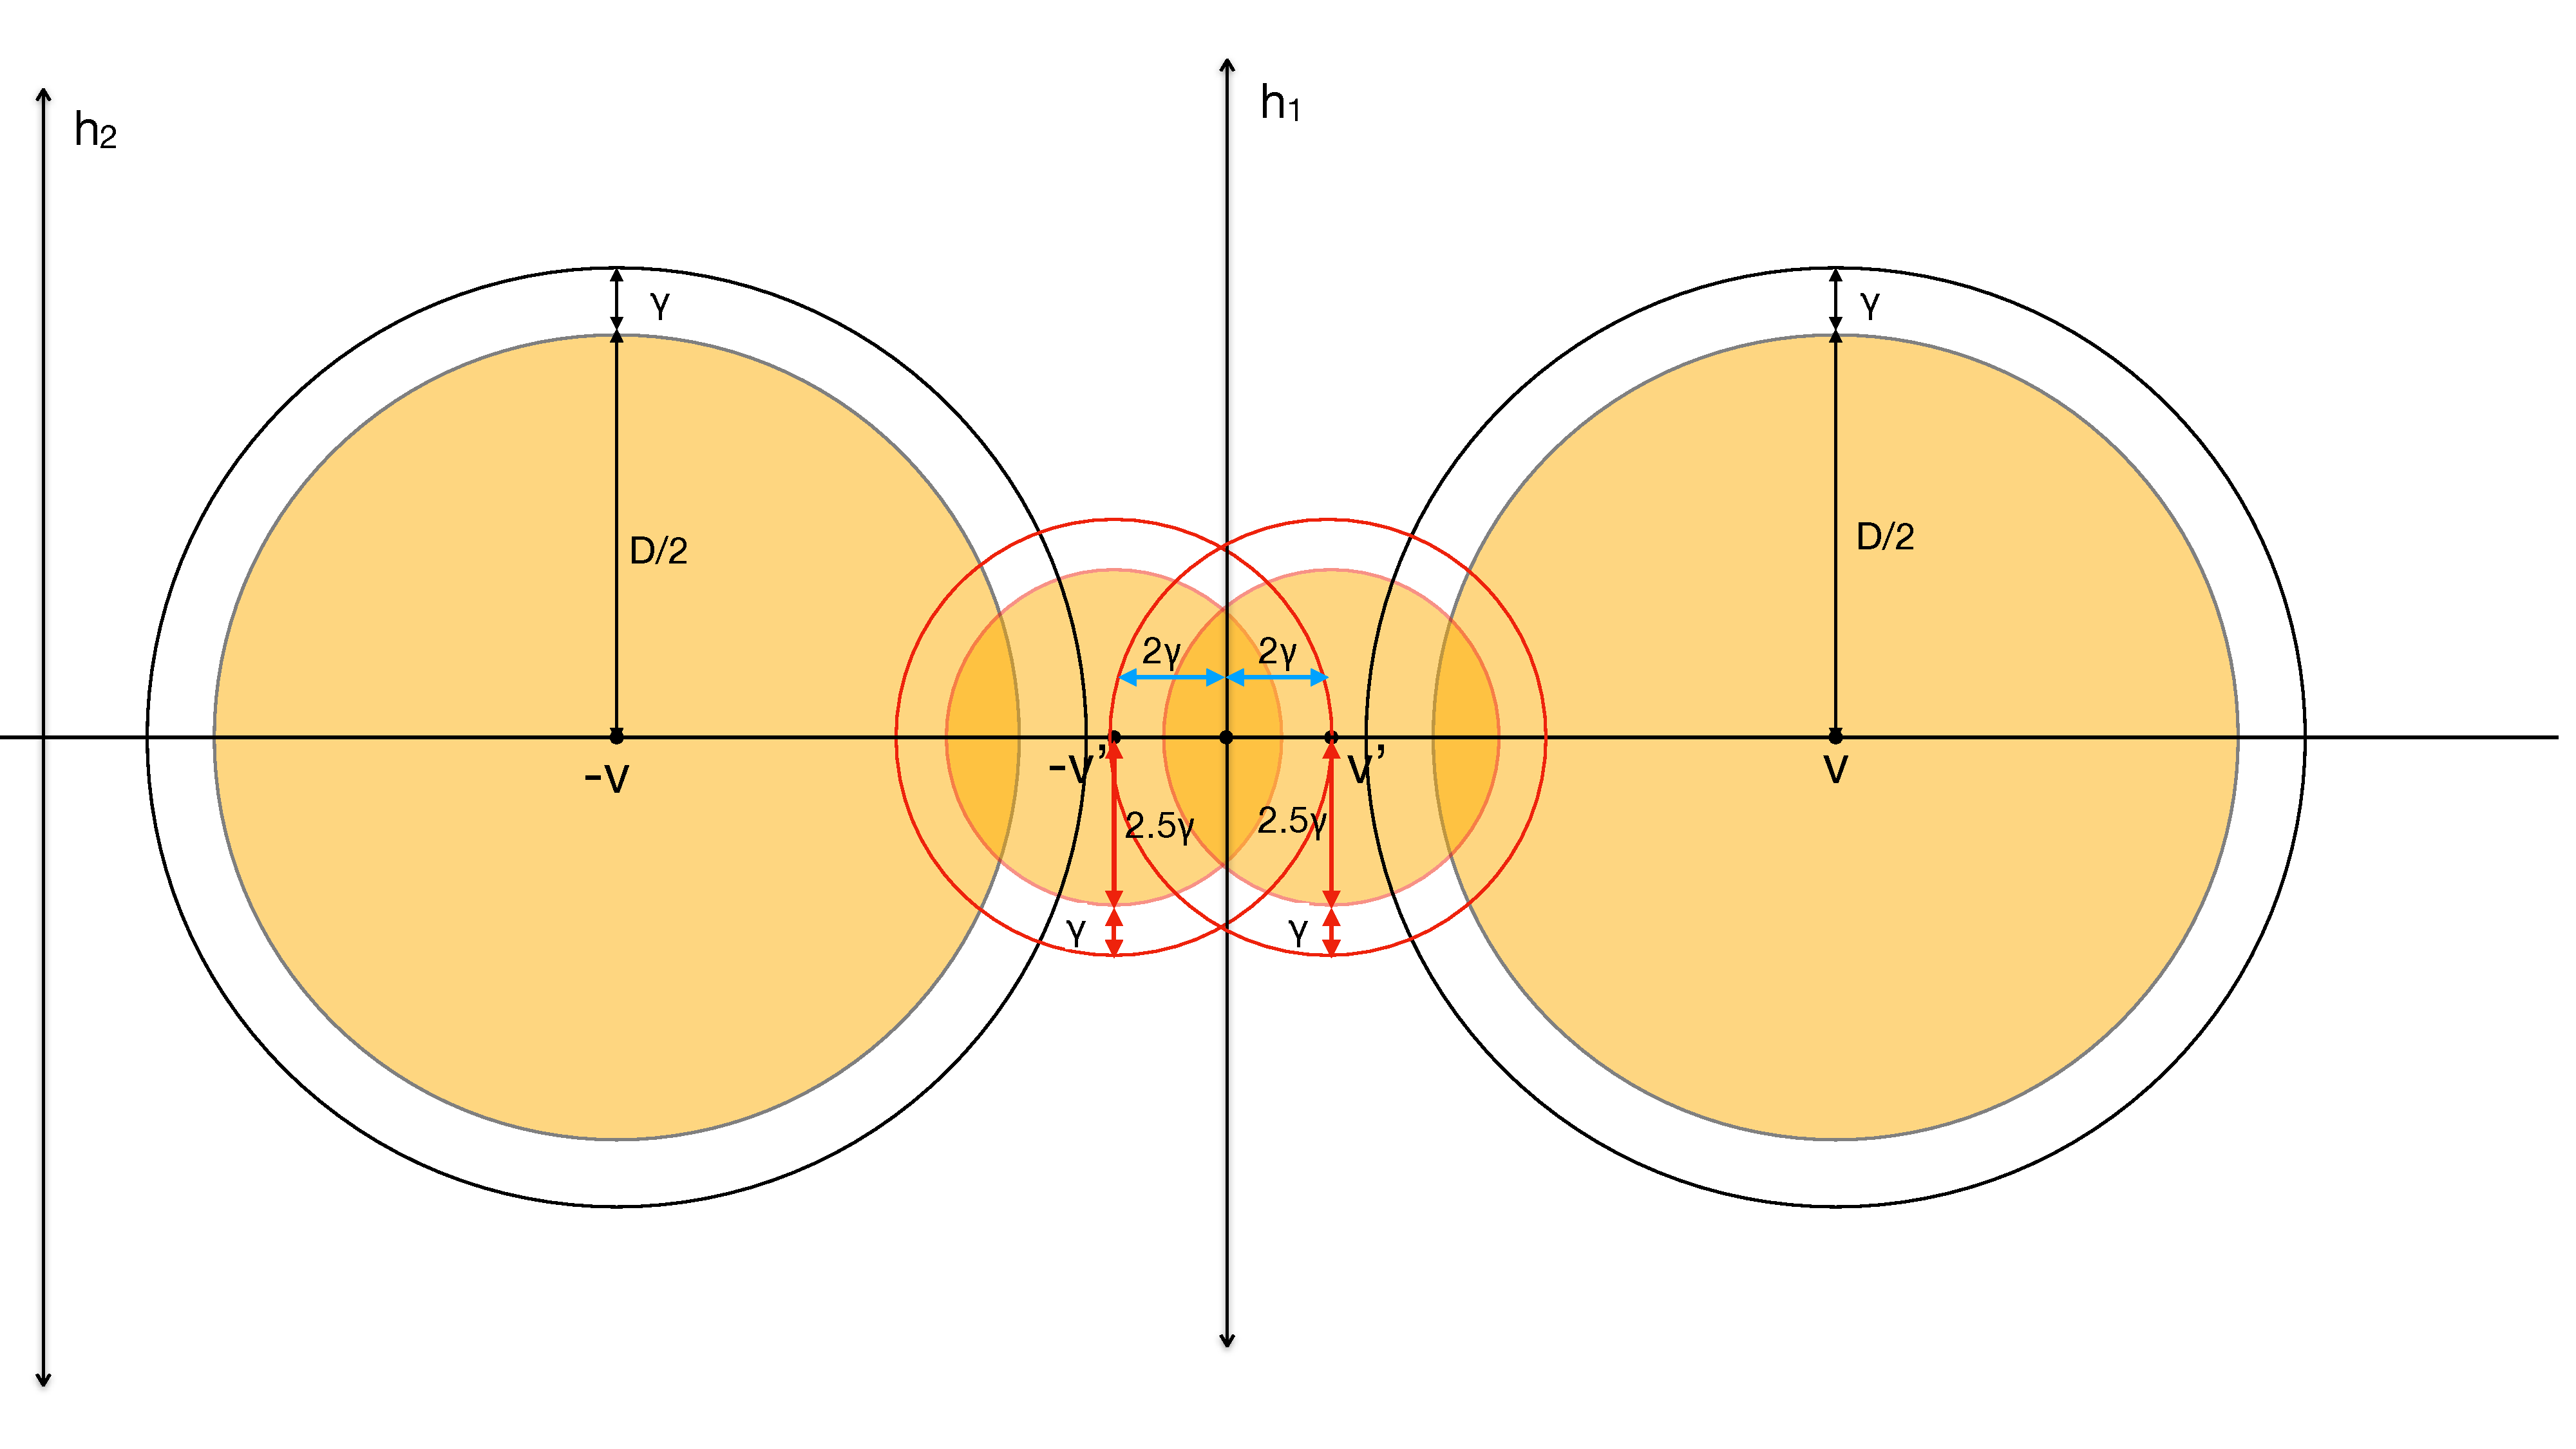
\includegraphics[width=.6\linewidth]{icml1.pdf}
	%	\caption{The generic task}
		\label{fig:LB}
	%\end{subfigure}
   \caption{Illustration for the sampling oracle lower bound in \propref{prop: lowerbound} in $\R^2$.}
	\label{fig:illustration}
\end{figure}

We now show a lower bound on the number of oracle calls required for tolerant learning in \citet{Urner22}'s sample oracle model. We first recall the model itself for completeness, focusing on the case of $(\mathbb{R}^d,\ell_2)$ endowed with the standard Lebesgue measure for simplicity.
\begin{defn}[Sampling Oracle {\cite{Urner22}}]
Let $U: \mathbb{R}^d \to P(\mathbb{R}^d)$ be any perturbation function such that $U(x)$ has finite Lebesgue measure for all $x \in \mathbb{R}^d$. The sampling oracle $\mathcal{O}_U$ inputs any $x \in \mathbb{R}^d$, and outputs a sample $y$ from the induced distribution on $U(x)$ under the Lebesgue measure.
\end{defn}
We prove that tolerant learning requires exponentially many calls to the sampling oracle.
\begin{customprop}{6}
For any $D>10\gamma > 0$, there exists a hypothesis class $\mathcal{H}$ and a set of robustness regions, $U$ such that the following holds. There exist constants $\epsilon$ and $\delta$ such that for any $n > 0$, any learner $L$ on $n$  samples that achieves 
$$\ell_U(L(S), \cD) \leq \min_{h \in \cH} \ell_{U^\gamma}(h, \cD) + \epsilon$$
with probability at least $1-\delta$ must make at least $\Omega\left(\left(\frac{D}{\gamma}\right)^d\right)$ calls to the sampling oracle for some valid data distribution $\cD$,
\end{customprop}
\begin{proof}[Proof of Proposition \ref{prop: lowerbound}]

Appealing to Yao's Minimax Principle, it is enough to find a class $\mathcal{H}$ and strategy for the adversary (over valid choices of perturbation sets and data distributions) such that any deterministic learner using at most $O((\frac{D}{\gamma})^d)$ oracle calls incurs at least constant error ($\epsilon$) over the optimum in $\mathcal{H}$ with constant probability ($\delta$). 

With this in mind, fix $D_0 =D-9\gamma$, let $r = 4\gamma$, and let $e_1$ denote the first canonical basis vector in $\R^d$. Our (marginal) data distribution will consist of two points in $\R^d$ $\curlybracket{(\frac{D_0}{2}+4\gamma)e_1,-(\frac{D_0}{2}+4\gamma)e_1}$. For the ease of notation, we denote $v \coloneqq (\frac{D_0}{2}+4\gamma)e_1$. Note, $||v- (-v)||_2 = D_0 + 2r$. We now define the underlying hypothesis class $\cH$ which consists of two linear classifiers $\cH \coloneqq \curlybracket{h_{1},h_{2}}$ such that $h_1 = sgn(\langle e_1, \cdot \rangle)$ and $h_2 = (\langle e_1, \cdot \rangle - D_0 - 4\gamma)$. Note that $h_1$ is a perpendicular bisector of the line segment joining $v$ and $-v$, and $h_2$ is parallel to $h_1$ but biased to the left of $v$.

Finally, we construct two perturbation sets with bounded diameter $U$ and $V$. Fix $v' = 2\gamma e_1$.
%points $v'$ and $-v'$ such that $v,v'$ are co-linear, $||x_1 - x_1'|| = \frac{D_0}{2} + 2\gamma$, and $||x_2 - x_2'|| = \frac{D_0}{2} + 2\gamma$. 
We define balls of radius $r>0$ for any given $x \in \R^d$ as $B_2(x, r)\coloneqq$ $\curlybracket{x' \in \R^d: ||x' - x||_2 \le r}$. First, we define a perturbation $U$ and its $\gamma$-perturbed region $U^\gamma$ as follows:
%Let the perturbation sets $U,V$ and their $\gamma$-perturbed sets for $\curlybracket{x_1,-v}$ be defined as 
\begin{gather*}
 U \coloneqq \curlybracket{U_{v},U_{-v}} \textnormal{where for any } x \in \curlybracket{v,-v}, U_{x} = B_2\paren{x, \frac{D_0}{2}},\\
 U^{\gamma}\coloneqq \curlybracket{U_{v}^\gamma,U_{-v}^\gamma} \textnormal{where for any } x \in \curlybracket{v,-v}, U_{x}^{\gamma} = B_2\paren{x, \frac{D_0}{2} +\gamma}
\end{gather*}
Similarly, we define another perturbation set $V$ and its $\gamma$-perturbed region $V^{\gamma}$:
\begin{gather*}
V\coloneqq \curlybracket{V_{v},V_{-v}} \textnormal{where for any } x \in \curlybracket{v,-v}, V_{x} = U_{x}\cup B_2\paren{x',\frac{5\gamma}{2}},\\
V^{\gamma}\coloneqq \curlybracket{V_{v}^\gamma,V_{-v}^\gamma} \textnormal{where for any } x \in \curlybracket{v,-v}, V_{x}^\gamma = U_{x}^\gamma \cup B_2\paren{x',\frac{7\gamma}{2}}
    %V \coloneqq \curlybracket{B\paren{x_1, \frac{D}{2}}\bigcup B\paren{x_1',\frac{5\gamma}{2}},B\paren{-v, \frac{D}{2}}\bigcup B\paren{x_2',\frac{5\gamma}{2}}}\\
 %V^{\gamma} \coloneqq \curlybracket{B\paren{x_1, \frac{D}{2}+\gamma}\bigcup B\paren{x_1',\frac{7\gamma}{2}},B\paren{x_2, \frac{D}{2}}\bigcup B\paren{x_2',\frac{7\gamma}{2}}}
\end{gather*}
where $x' = v'$ or $-v'$ if $x = v$ or $-v$ respectively. We assume that the perturbation set for $\R^d\setminus \curlybracket{v,-v}$ is null for simplicity. 
Observe that $\bigcap\limits_{x' \in \curlybracket{v,-v}} U_{x'} = \emptyset$ and so is the intersection of perturbations in $U^\gamma$.
%First, we note that $V$ is a $\gamma$-\textbf{perturbed regions} of $U$.
But, we note that $\bigcap\limits_{x' \in \curlybracket{v,-v}} V_{x'} \not= \emptyset$. This entire construction is illustrated in Figure \ref{fig:illustration}.
%Furthermore, we can pick $p_0$ such that the measure of the intersection of the sets $V^{\gamma}_{x_1}$ and $V^{\gamma}_{x_2}$ is upper bounded by $\paren{\frac{\gamma}{D}}^d$, i.e. $\mu\paren{V^{\gamma}_{x_1}\cap V^{\gamma}_{x_2}} \le \paren{\frac{\gamma}{D}}^d$.
% As considered in \citet{Urner22}, for a perturbation set $Z = U$ or $Z = V$, a sampling oracle samples based on the induced probability measure $P_{Z_x}^{\mu}$ over $Z_x \in Z$ as follows. For any set $Z'\subseteq Z_x$ in the $\sigma$-algebra over $Z_x$, we define 
% $P_{Z_x}^{\mu}(Z') = \frac{\mu(Z')}{\mu(Z_x)}$.

We are now ready to describe the adversary's strategy, who chooses one of $U$ or $V$ independently with probability $1/2$, and employs a single fixed choice of data distribution $\cD$ where $\Pr[Y = -1 | -v] = \Pr[Y = 1 | v] = 1$, and the marginal distribution is uniform over $v$ and $-v$. Note that if the perturbation set is $U$, then $h_1$ is optimal as $\ell_U\paren{h_1,\cD} = 0$ whereas $\ell_U\paren{h_2,\cD} = 1/2$. On the other hand if $V$ is chosen then $h_2$ is optimal as $\ell_V\paren{h_2,\cD} = \frac{1}{2}$ and $\ell_V\paren{h_1,\cD} = 1$. The idea is to show that the learner cannot distinguish between $U$ and $V$ with high probability, and thus cannot choose the right hypothesis. We note that since the data distribution is fixed and known to the learner, we only need to consider randomness over the sample oracle---labeled samples have no effect on the bound.

More formally, we split our analysis into two cases based on whether or not the learner draws an (oracle) sample in $V^\gamma \setminus U^\gamma$. First, note that conditioned on the fact that the learner draws no such sample, by construction the posterior probability of $U$ is strictly higher than that of $V$. This means the learner's expected excess error is minimized by always outputting $h_1$ on such samples. On the other hand, if the learner observes a sample in $V^\gamma \setminus U^\gamma$, they can always achieve optimal error by outputting $h_2$. 

Since the above learning rule minimizes the learner's expected excess error, it is enough to bound the expected error of this rule:
\begin{align*}
    \mathbb{E}_{Z,S \sim \mathcal{O}_Z}[OPT_Z - \ell_{Z}(\mathcal{A}(S),\cD)] &\geq \frac{1}{2}\Pr[S \subset U^\gamma \wedge Z=V]\\
    &= \frac{1}{2}\Pr[Z=V]\Pr[S \subset U^\gamma | Z=V]\\
    &= \frac{1}{4}\Pr[S \subset U^\gamma | Z=V]
\end{align*}

The key observation is then simply to notice that $\Pr[S \subset U^\gamma | Z=V]$ is constant whenever the learner draws at most $O((\frac{D}{\gamma})^d)$ oracle samples. This follows from the fact that under the induced distribution $P_{V^\gamma}$ on $V$:
\begin{equation}
 P_{V^\gamma}(V^\gamma\setminus U^\gamma) = \frac{\mu(V^\gamma\setminus U^\gamma)}{\mu(V^{\gamma})} \le \frac{\mu(B_2(v',\frac{7\gamma}{2}))}{\mu(U^\gamma_v) + \mu(B_2(v',\frac{7\gamma}{2}))} \le \frac{(\frac{7}{2}\gamma)^d}{D_0^d}\nonumber
\end{equation}
where $\mu$ is the standard Lebesgue measure. Similarly we then have
\begin{align*}
    P_{V^\gamma}(U^\gamma) \ge 1 - \frac{(\frac{7}{2}\gamma)^d}{D_0^d} \label{eq: U}
\end{align*}
and finally that
\begin{align*}
    \Pr[S \subset U^\gamma | Z=V] \geq \paren{1 - \frac{(\frac{7}{2}\gamma)^d}{D_0^d}}^{|S|}
\end{align*}
which is at least some constant when $|S| \leq c(\frac{D_0}{\gamma})^d$ for some sufficiently small absolute constant $c<0$. Since $D_0 = D - 9\gamma$, there exists $c'$ such that this holds when $|S| \leq c'(\frac{D}{\gamma})^d$ which implies the proposition.
% the probability the learner draws no sample in $V^\gamma \setminus U^\gamma$ is high.

% Fix a training sample of size $N$, say $S_N \coloneqq \curlybracket{(x_i,y_i)}_{i=1}^N$ such that the learner calls the sampling oracle for less than $Q_N = \paren{\frac{D}{\gamma}}^d$ times.

% Now, if the adversary picks the perturbation set to be $U$, then we know that the sampling oracle can sample only from $U^\gamma$. In this case, note that as the sampling oracle provides a perturbed sample from $U^\gamma$ the learner could correctly pick the optimal hypothesis $\hat{h}\coloneqq h_1$ as it distinguishes $U$ from $V$. Thus, the expected error $\ell_U(\hat{h},\cD) = 0$ if learner picks $\cA^\gamma(S_N) = h_1$, otherwise $\ell_U(h_2,\cD) = \frac{1}{2}$. 

% Consider the case that the adversary picks $V$ as the perturbation set. The sampling oracle can sample perturbed points from $V^\gamma$. First, note that for all $x \in \curlybracket{v,-v}$, $U_x^\gamma \subset V_{x}^\gamma$. Thus, it is possible that the sampling oracle samples perturbed points only from $U^\gamma$. If that is the case, then $\ell_V(\hat{h},\cD) = 1$ if $\cA^{\gamma}(S_N) = h_1$. But in case if the algorithm picks $\cA^\gamma(S_N) = h_2$ then $\ell_V(\hat{h},\cD) = \frac{1}{2}$. But then $\ell_U(\hat{h},\cD) = \frac{1}{2}$ because sampling oracle only sampled from $U^\gamma$. %Thus, the expected error over the choice of perturbation sets is $\frac{1}{2}\ell_U(\hat{h},\cD) + \frac{1}{2}\ell_V(\hat{h},\cD) \ge \frac{1}{2}$ if oracle picks points from $U^\gamma$.

% Now, consider that the sampling oracle picks perturbed points from $V^\gamma\setminus U^\gamma$. If $\cA^\gamma(S_N) = h_1$ then $\ell_V(\cA^\gamma(S_N),\cD) = 1$, otherwise $\ell_V(\cA^\gamma(S_N) = h_2,\cD) = \frac{1}{2}$. Thus, in order to minimize the error, $\cA^{\gamma}$ chooses $h_2$ upon given the training sample $S_N$.% and thus the total error $\frac{1}{2}\ell_U(\hat{h},\cD) + \frac{1}{2}\ell_V(\hat{h},\cD) = \frac{1}{4}$. 

% Note that sampling oracle can sample a perturbed point in $V^\gamma\setminus U^\gamma$ with probability
% \begin{equation}
%  P_{V^\gamma}^{\mu}(V^\gamma\setminus U^\gamma) = \frac{\mu(V^\gamma\setminus U^\gamma)}{\mu(V^{\gamma})} \le \frac{\mu(B_2(v',\frac{7\gamma}{2}))}{\mu(U^\gamma_v) + \mu(B_2(v',\frac{7\gamma}{2}))} \le \frac{(\frac{7}{2}\gamma)^d}{D^d}\nonumber
% \end{equation}
% Similarly,
% \begin{align}
%     P_{V^\gamma}^{\mu}(U^\gamma) \ge 1 - \frac{(\frac{7}{2}\gamma)^d}{D^d} \label{eq: U}
% \end{align}
% %Note that in order to sample for $V^\gamma\setminus U^\gamma$, sampling oracle has to sample perturbed examples from $V_{x_1}^{\gamma}\cap V_{x_2}^{\gamma}$. We know that $\mu\paren{V^{\gamma}_{x_1}\cap V^{\gamma}_{x_2}} \le \paren{\frac{\gamma}{D}}^d$. 
% If $Q_N \le \frac{D^d}{(\frac{7}{2}\gamma)^d}$, then using \eqref{eq: U} there is a non-trivial constant probability $p_0 > 0$ that sampling oracle picks points in $U^\gamma$. Now, we can bound the expected error over randomized choices of perturbation set as follows:
% \begin{align}
%     \expctover{S_N}{\expctover{Z\sim(U,V)}{\ell_Z(\cA^\gamma(S_N),\cD)}} &\ge P_{\cD}(\textnormal{\textbf{1}}\curlybracket{S_N \sim U^\gamma})\cdot\paren{\frac{1}{2}\ell_U(\cA^\gamma(S_N),\cD) + \frac{1}{2}\ell_V(\cA^\gamma(S_N),\cD)}\label{eq: bound1}\\
%     &\ge p_0\cdot\paren{\frac{1}{4} + \frac{1}{4}}\label{eq: bound2}\\
%     &= \frac{p_0}{2}\nonumber
% \end{align}
% In \eqnref{eq: bound1}, we consider the samples $S_N$ that fall in $U^\gamma$. In \eqnref{eq: bound2}, we note that if $\cA(S_N) = h_1$ then the expected error is $\frac{1}{2}\ell_U(h_1,\cD) + \frac{1}{2}\ell_V(h_1,\cD) \ge \frac{1}{2}$. In case, $\cA^\gamma(S_N)= h_2$ then the expected error is $\frac{1}{2}\ell_U(h_2,\cD) + \frac{1}{2}\ell_V(h_2,\cD) \ge \frac{1}{4} + \frac{1}{4} = \frac{1}{2}$. This implies that the randomized algorithm forces a lower bounded error for any deterministic tolerant algorithm $\cA^\gamma$ if $Q_N \le \frac{D^d}{(\frac{7}{2}\gamma)^d}$.
%%%%%%%%%%%%%%
%But then $\cA^\gamma$ incurs at least error $c_0\ell_V(\hat{h},\cD) > \frac{c_0}{2}$ with constant probability over the choice of $S_N$. Using Yao's minimax theorem, total expected costas argued above the total error is at least $\frac{1}{2}$ with constant probability. which implies that the tolerant algorithm $\cA^\gamma$ is forced to call the sampling oracle at least $\paren{\frac{D}{\gamma}}^d$ times in order to distinguish $V$ from $U$ in order to incur optimal error with high probability. Given that the tolerant algorithm $\cA^\gamma$ calls sampling oracle for less than $\paren{\frac{D}{\gamma}}$The probability that the sampling oracle picks points from $U^\gamma$,It is evident that to distinguish $V$ from $U$, sampling oracle needs to sample examples from $V^\gamma \setminus U^\gamma$ when the adversary picks $V$, otherwise the total error is at least $\frac{1}{2}$. 
%%%%%%%%%%%%%
%Otherwise the learner will choose $h_1$ for $V$, and incurs an expected loss of $\frac{1}{2}\times\ell_V(h_1,\cD) = \frac{1}{4}$ \textcolor{red}{HY: Again, should $\ell_V(h_1,\cD) = 1?$} and vice versa. \textcolor{red}{HY: What does vice versa mean here? When the adversary chooses $U$?}
%Irrespective of the hypothesis returned by any tolerant algorithm, adversary could also pick the perturbation set that leads to a wrong optimal.
 


%\begin{align*}
%    \expctover{Z \sim \paren{U,V}}{\ell_Z(\hat{h},\cD)} = \frac{1}{2}\ell_U(\hat{h},\cD) + \frac{1}{2}\ell_V(\hat{h},\cD)
%\end{align*}

\end{proof}

We note that in \citet{Urner22}, the sampling oracle is defined more generally for any \textit{doubling-measure} $\mu$, that is any measure for which there exists some ``doubling-constant'' $C>0$ such that for all $x \in \mathbb{R}^d$ and $r \in \mathbb{R}^+$:
\[
0 < \mu(B(x,2r)) \leq C\mu(B(x,r)) < \infty.
\]
In this more general setting, one can prove a lower bound that scales with the doubling-constant (typically exponential in the associated doubling-dimension of the metric space) simply by appropriately increasing the concentration of measure on $U^\gamma$. 


\section{Robust VC for $k$ points}\label{app: robust vc bound}
In this section, we prove that the size-$k$ perturbation sets only cost a $\log(k)$ factor over the VC dimension of the original class. To formalize this, we first recall a few basic definitions standard to the (adversarially robust) learning literature.

\begin{defn}[Robust Loss Class]
Given a hypothesis $h: \cX \to \{0,1\}$ and perturbation function $U:\cX \to P(\cX)$, let $h^\ell_U: X \times \{0,1\}$ be the function over labeled samples measuring the robust loss of $h$:
\[
h^\ell_U(x,y) = \begin{cases}
0 & \text{ if } \ \forall x' \in U(x): h(x')=y\\
1 & \text{ else.}
\end{cases}
\]
The robust loss class of $(\cX,\cH)$ is the hypothesis class over $\cX \times \{0,1\}$ given by:
\[
\mathcal{L}^U_{\cH} \coloneqq \{ h^\ell_U : h \in \cH\}.
\]
\end{defn}
We are interested in analyzing a standard complexity measure of the robust loss class called VC dimension
\begin{defn}[VC Dimension]
The VC dimension of a hypothesis class $(\cX,\cH)$ is the size of largest subset $S \subseteq \cX$ such that $\cH$ obtains all $2^{|S|}$ labelings on $S$. We say such a set is \textit{shattered} by $\cH$.
\end{defn}
% We define the robust VC dimension of a class $(X,H)$ as the VC dimension of its robust loss class.
% \begin{defn}[Robust VC Dimension]
% The robust VC dimension of a hypothesis class $(X,H)$ with respect to perturbation function $U:X \to P(X)$ is $vc(\mathcal{L}^U_H)$.
% \end{defn}
We show the VC dimension of the robust loss class incurs at most $\log(k)$ blow-up over the original class.
\begin{prop}[Overhead of Robust VC]\label{prop:finite-RVC}
Let $(\cX,\cH)$ be a hypothesis class of VC-dimension $d$ and $U: \cX \to P(\cX)$ any perturbation function with support bounded by some $k \in \mathbb{N}$. Then the VC dimension of $\mathcal{L}^U_{\cH}$ is at most $O(d\log(dk))$.
\end{prop}
This result was also independently communicated to us by Omar Montasser. The proof of Proposition \ref{prop:finite-RVC} relies on the classical Sauer-Shelah-Perles lemma, which we recall here for completeness.
\begin{lem}[Sauer-Shelah-Perles \cite{sauer1972density,shelah1972combinatorial}]
Let $(\cX,\cH)$ be a hypothesis class of VC-dimension $d$. Then for any finite subset $S \subseteq \cX$, $\cH$ obtains at most $O(|S|^d)$ distinct labelings on $S$.
\end{lem}
Proposition \ref{prop:finite-RVC} simply follows from using Sauer-Shelah-Perles to bound the total number of permissible patterns across perturbation sets of a sample in the loss space.
\begin{proof}[Proof of Proposition \ref{prop:finite-RVC}] Let $m \in \mathbb{N}$ and assume there exists a sample $S=(x_1,y_1), \ldots, (x_m,y_m)$ that is shattered by $\mathcal{L}^U_{\cH}$. We will show $m \leq O(d\log(kd))$. With this in mind, let $T=\bigcup_{i=1}^m U(x_i)$ denote the set of at most $km$ points corresponding to the robustness regions of our sample. The key observation is the following (essentially trivial) claim:
\begin{claim}
Any two $g_{U}^\ell,h_{U}^\ell \in \mathcal{L}^U_{\cH}$ that give distinct labelings of $S$ correspond to $g,h \in \cH$ with distinct labelings of $T$.
\end{claim} 
By robust shattering, there exist $2^m$ distinct labelings of $S$ by $\mathcal{L}^U_{\cH}$, so the above claim implies $\cH$ must have $2^m$ distinct labelings of $T$. However the latter has at most $O((km)^d)$ labelings by VC dimension, so
\[
2^m \leq O((km)^d) \Rightarrow m \leq O(d\log(dk))
\]
by standard manipulations. Finally, we note the claim is immediate from definition, since the behavior of a function $h_U^\ell \in \mathcal{L}^U_{\cH}$ on $S$ depends only on the labels of its corresponding hypothesis $h \in \cH$ on $T$ by definition. 
\end{proof}

\section{Proof of Theorem \ref{thm:upper_bound_general}}\label{sec:proof_extension}

We begin by defining $v_{ball}$, which is the adversarial VC dimension when the robustness regions are all balls of a fixed radius. We start by precisely defining these robustness regions. 

\begin{defn}
Let $U^r$ be the set of robustness regions defined by $\{U_x^r = B(x, r)\}$, where $B(x, r)$ denotes the closed ball of $\ell_2$-radius $r$ centered at $x$. 
\end{defn}

We now define the adversarial VC dimension of a set of classifiers $\cH$ for a fixed set of regions, $U^r$.

\begin{defn}
Let $\cH$ be a set of classifier. Then the adversarial VC dimension of $\cH$ with respect to $U^r$ is the maximum integer $v$, for which there exist $v$ labeled points, $(x_1, y_1), \dots, (x_r, y_r)$ so that for any subset $S \subset \{(x_1, y_1) ,\dots, (x_r, y_r)\}$, there exists $h_S \in \cH$ with $$\ell(h_S, (x_i, y_i) = \begin{cases}0 & i \in S \\ 1 & i \notin S\end{cases}.$$ We denote this by $v_{ball}^r$.
\end{defn}

Finally, we define $v_{ball}$ as the maximum value of $v_{ball}^r$ over all $r > 0$. Note that this quantity has been well studied -- for example \cite{Cullina18} shows that for linear classifiers, $v_{ball} = O(d)$. 

\paragraph{Proving Theorem \ref{thm:upper_bound_general}} We now turn our attention towards the proof. The key observation is that the main steps from the proof of Theorem \ref{thm:upper_bound1} \textit{perfectly} carry over. In particular, Lemma \ref{lem:r_works} exactly holds in this setting, and the argument given in the proof of Theorem \ref{thm:upper_bound1} also holds provided that an appropriate choice of $V$ exists. The only issue arises from Lemma \ref{lem:v_construct}, which requires that $\cH$ be regular. To remedy this, we now state and prove a different version of this lemma that uses a union of balls (of fixed radius) for $V_x$ rather than a finite set of points. 

\begin{lem}\label{lem:v_construct_new}
Let $\cH$ by an arbitrary hypothesis class. For all $r \in [\frac{\epsilon\delta\gamma}{7}, \gamma]$, let $\alpha$, $U^r$ and $U^{r-\alpha}$ be as described in the proof of Theorem \ref{thm:upper_bound1}. Then there exists a set of robustness regions $V^r = \{V_x^r: x \in \reals^d\}$ satisfying the following two properties.  
\begin{enumerate}
	\item $V_x^r$ is a union of $O\left(\left(\frac{D}{\epsilon\delta\gamma}\right)^d\right)$ balls of radius , where $D$ denotes the maximum diameter of $U_x$. 
	\item Let $\alpha = \frac{\epsilon\delta\gamma}{7}$. For all labeled points $(x,y)$ and for all classifiers $h \in \cH$, $$\ell_{U^{r - \alpha}}(h, (x,y)) \leq \ell_{V^r}(h, (x,y)) \leq \ell_{U^r}(h, (x,y)).$$
\end{enumerate}
\end{lem}

\begin{proof}
Since $U_x^{r-\alpha}$ has diameter at most $D$, it follows that it can be covered with $O\left(\left(\frac{D}{\epsilon\delta\gamma}\right)^d\right)$ balls of radius $\frac{\alpha}{2}$. We let $V_x^r$ be any such cover that is minimal (meaning that (1.) is satisfied), meaning that each ball intersects $U_x^{r-\alpha}$. It follows that for all $x$, $U_x^{r-\alpha} \subseteq V_x^r \subseteq U_x^r$, which immediately implies (2.) and completes the proof. 
\end{proof}

Finally, to prove Theorem \ref{thm:upper_bound_general}, we note that the proof of Theorem \ref{thm:upper_bound1} essentially works. The only differences are that instead of bounding the robust VC dimension of $\cH$ with respect to $V_X$ in terms of $v$, we must use $v_{ball}$ as we are now considering unions of balls rather than points. As a detail, note that we are using the following minor modification of Proposition \ref{prop:finite-RVC} to bound the robust VC dimension of unions of balls using the robust VC dimension for balls. 
\begin{prop}
Let $(\cX,\cH)$ be a hypothesis class whose robust loss class with respect to $r$-balls has VC dimension $v_{\text{ball}}^r$. Then the loss class of $(\cX,\cH)$ with respect to perturbations that are a union of at most $k$ $r$-balls has VC dimension at most $O(v_{\text{ball}}^r\log(v_{\text{ball}}^rk))$.
\end{prop}
\begin{proof}
The proof is largely the same as \ref{prop:finite-RVC}. Denote the original perturbation family as $U$, and the $k$-union perturbation family by $U^k$. Given a sample $S=(x_1,y_1),\ldots,(x_m,y_m)$, let $C_i$ denote the centers of the at most $k$ balls appearing in the perturbation set of $x_i$. It is enough to observe that any two distinct labelings of $S=(x_1,y_1),\ldots,(x_m,y_m)$ by $\mathcal{L}^{U^k}_{\cH}$ correspond to distinct labelings of the extended sample $T=\bigcup_{i=1}^m (C_i,y_i)$ with respect to $\mathcal{L}^{U}_{\cH}$, where $(C_i,y_i)$ denotes the sample $\bigcup_{c \in C_i} (c,y_1)$. The bound then follows from the same double counting argument as in Proposition \ref{prop:finite-RVC}.
\end{proof}












 